\section{\uppercase{Experimental results}}
\label{sec:results}
\subsection{Data} \label{sec:unitroot}
AVECM tests were carried out using four foreign exchange rates all related to
USD: EURUSD, GBPUSD, USDCHF and USDJPY. This data was collected from Dukascopy~\cite{Dukascopy2014}, a free
database which gives access to the Swiss Foreign Exchange marketplace.

The tests were done using 10-seconds frequency from ask prices
from the 11th to the 15th of August 2014. Since one day corresponds to 8640 data points and we used 5 days of data, we have 43,200 data points in total.

\subsection{Unit root tests} \label{sec:unitroot}

VECM can only be used if the time series are I(1). Therefore, 
before running the tests, we firstly checked whether the time series were
I(1) using the Augmented Dickey Fuller (ADF) test with lags $p=1,2,3,4,5$. 
MacKinnon \cite{mackinnon2010} critical values for rejection of hypothesis of a unit root are: -2.62 (1\%), 1.94 (5\%) and 1.62 (10\%).
\begin{table*}[ht]
\label{tab:adf}
\centering
\begin{tabular}{llllll}
\toprule
{Variable} & {ADF(1)} & {ADF(2)} & {ADF(3)} & {ADF(4)} & {ADF(5)}\\ 
\midrule
EURUSD &  -0.052   & -0.054  & -0.054  & -0.054  & -0.054  \\
GBPUSD &  -0.744  & -0.784  & -0.805  & -0.837  & -0.846  \\
USDCHF &  -0.476   & -0.493  & -0.493  & -0.495  & -0.502  \\
USDJPY &  0.357   & 0.360  & 0.360  & 0.367  & 0.367  \\
$\Delta$ EURUSD & -128.4*  & -128.4*  & -96.85* & -89.12*   & -89.12*\\
$\Delta$ GBPUSD & -131.4*  & -112.7*  & -102.5* & -92.86*   & -88.29*\\
$\Delta$ USDCHF & -127.8*  & -127.8*  & -96.94* & -88.82*   & -80.79*\\
$\Delta$ USDJPY & -135.1*  & -135.1*  & -101.2* & -101.2*   & -101.2*\\
\bottomrule
\addlinespace[1ex]
\multicolumn{6}{l}{ \textsuperscript{*} Indicates significance at 1\% level} \\
\multicolumn{6}{l}{ \textsuperscript{**} Indicates significance at 5\% level} \\
\multicolumn{6}{l}{ \textsuperscript{***} Indicates significance at 10\% level} \\
\multicolumn{6}{l}{MacKinnon critical values for rejection of hypothesis of a unit root are:}\\
\multicolumn{6}{l}{ -2.62 (1\%), -1.94 (5\%) and -1.62 (10\%)}\\
\multicolumn{6}{l}{ADF($d$) Augmented Dickey-Fuller test with lag $d$} 
\end{tabular}
\caption{Unit roots tests for EURUSD, GBPUSD, USDCHF and USDJPY at 10-seconds
frequency.}
\end{table*}
Table~\ref{tab:adf} shows that all currency rates cannot reject the unit root test in their level form considering different lags, but they rejected it with their first differences. This means that all of
them are I(1) time series and we are allowed to use VECM and therefore our proposed AVECM.

\subsection{Performance accuracy} \label{sec:performance}

Algorithms AVECM, ARIMA and the naive random walk were tested using four days of data (from the 12th to the 15th of August 2014).
For AVECM we considered different number of iterations (parameter $m$ in algorithm \ref{alg:AVECM}): 10, 50 and 100. We tried 12, 24 and 47 different pair of combinations for $L$ and $p$. Possible values for $L$ were in the interval $[100,4000]$ and $p$ can have values in between $[1,5]$. Best AVECM performance was compared against ARIMA and the random walk model.
Table~\ref{tab:stats} shows the out-of-sample performance measures: MSE and $U$-statistic for AVECM and ARIMA. In terms of both measures we found that AVECM is superior to ARIMA and the naive random walk model. We also included the p-value that proves that the difference in the MSE is significant at the 99\% significance level in three of the four currency rates and at 90\% in the case of GBPUSD. The $U$-statistic shows that AVECM and ARIMA are superior to the naive random walk model and that our proposal is also superior to ARIMA.

\begin{table}[!htbp]
\caption{AVECM performance}
\label{tab:stats}
\begin{center}
\begin{tabular}{ccccccc}

& \multicolumn{3}{l}{MSE} & &
\multicolumn{2}{c}{$U$-statistic} \\ 
\hhline{~---~--} \\
 &
AVECM & ARIMA & p-value & &
AVECM & ARIMA \\ 

\hline
 EURUSD & 1.0702 e-09 & 1.1481 e-09 &  9.2509 e-12 & & 0.6863 & 0.7108\\
 GBPUSD & 1.6630 e-09 & 1.7408 e-09 &  6.9519 e-02 & & 0.6866 & 0.7025\\
 USDCHF & 5.8503 e-10 & 6.3545 e-10 &  2.8999 e-14 & & 0.6803 & 0.7091\\
 USDJPY  & 6.3483 e-06 & 6.5194 e-06 &  6.8536 e-05 & & 0.6964 & 0.7057\\
 \end{tabular}
 \end{center}
\end{table}

\subsection{Parallel implementation} \label{sec:parallel}

To determine $L$ and $p$ based on maximising the percentage of cointegration requires use of the 
Johansen
method which is a computationally expensive routine. This procedure is done by the function get\_best\_params($Ls,ps,m,\mathbf{Y}$) shown in algorithm \ref{alg:AVECM}.
In order to improve the execution time of this search, our proposal included
a parallel search of VECM parameters using high performance computing.
The main objective was to obtain a response before a new data arrived in
the following10 seconds.

The Johansen method is already programmed in the Python Statsmodels
library~\cite{seabold2010} and the parallel implementation was developed using
MPI in Python. 
We chose MPI because it allows large-scale parallel applications
with wide portability to be built, being able to run in large clusters
or on local computers.
We tested our proposal in a cluster with 2 servers Xeon E5-2667 (2.90GHz)
of 24 cores each (48 cores in total) and 24GB RAM.
In order to compare serial and parallel execution times in AVECM, we set parameter $it=100$ in algorithm\ref{alg:AVECM}.

The $L$ parameter was always chosen between 100 and 4000 and $p$ always took values
between 1 and 5. Parameter $nparams$ represents the number of pairs ($L$,$p$) used to maximise the percentage of cointegration. 

Execution time depends directly on $L$, $p$ and $nparams$ used, since they determine the size of
matrix $\mathbf{A}$ (see equation \ref{eq:Amatrix}) and therefore affect the OLS function execution time.
Therefore, if we try more combinations of $L$ and $p$ (increasing $nparams$) the
serial algorithm will take longer. For this financial time series we are interested in execution times below 10 seconds  (the time series frequency).

\begin{figure}[ht]
  \centering
  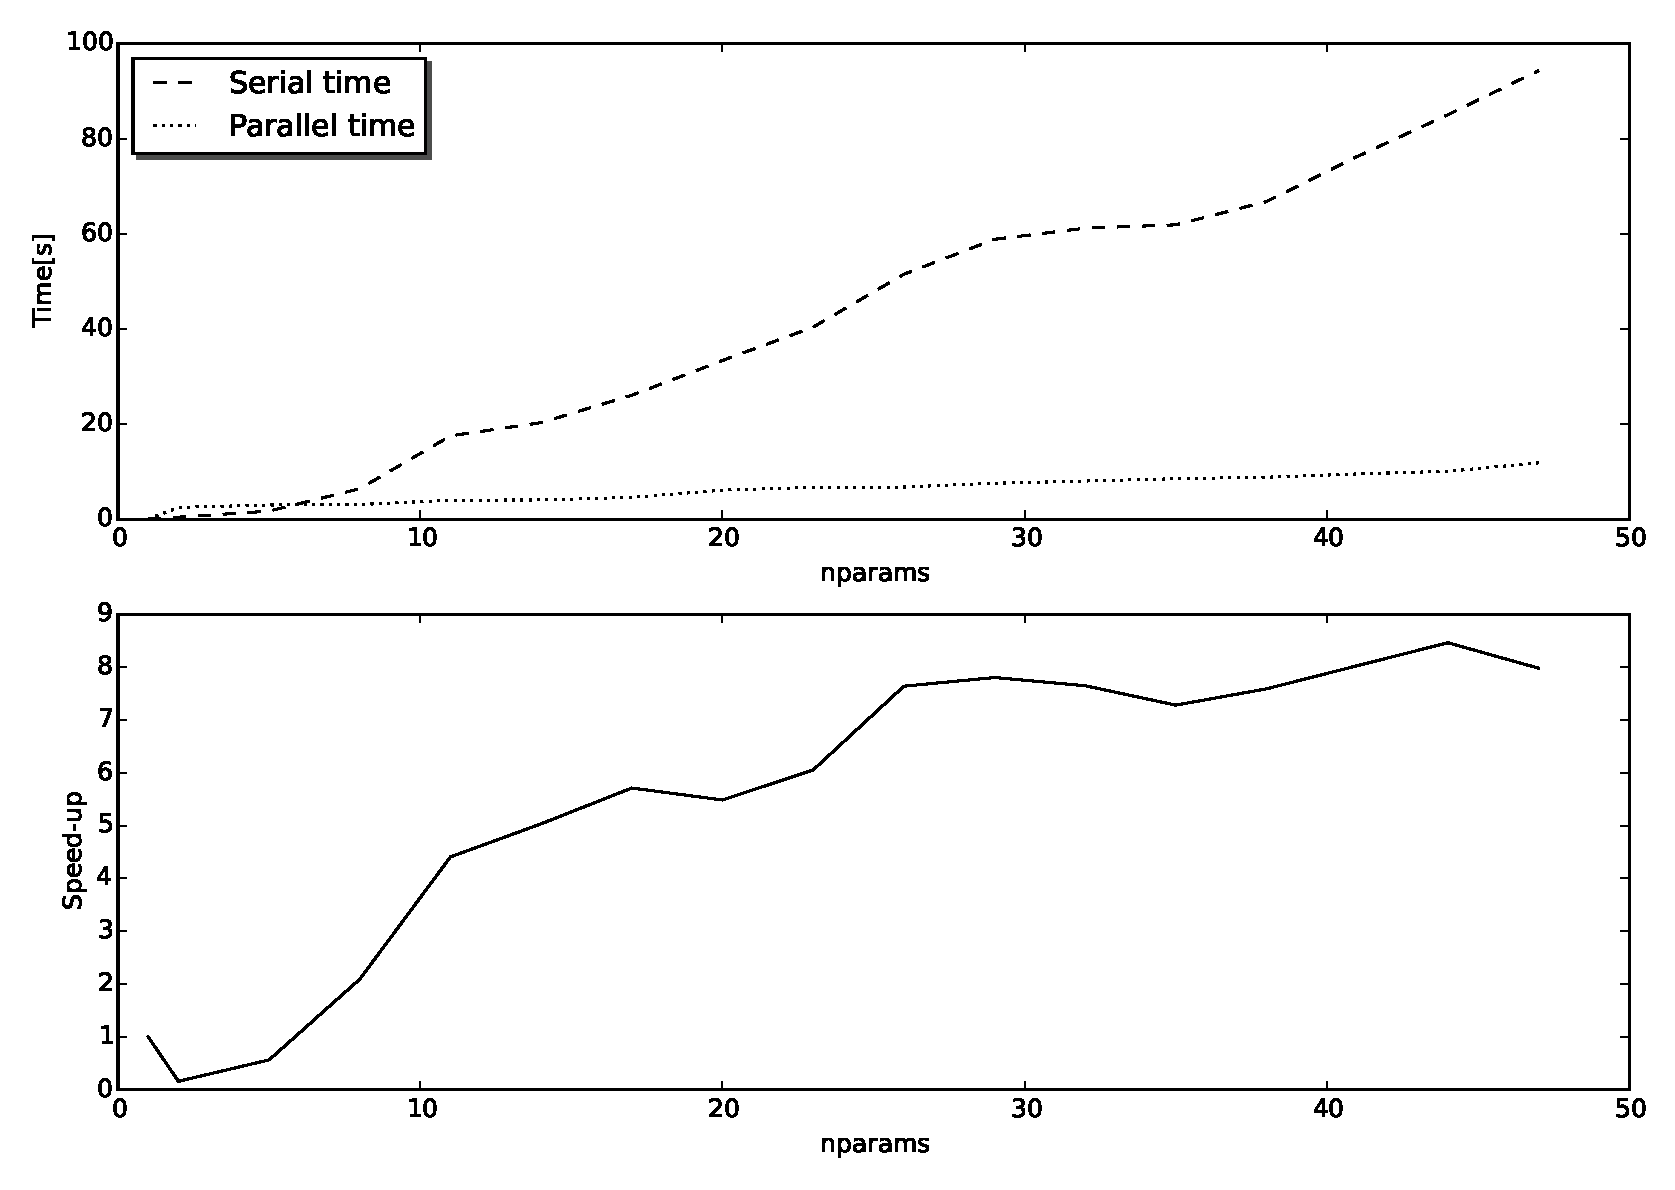
\includegraphics[width=0.75\textwidth]{img/extimes}
  \caption{Computing time of sequential and parallel algorithm is shown in the
  upper figure. Speed-up is shown below.}
  \label{fig:extimes}
\end{figure}

The superior figure \ref{fig:extimes} shows that best performance accuracy measurements are
achieved in times near or below 10 seconds in the parallel version. Contrarily,
serial times are high, above 10 seconds in most cases. Figure~\ref{fig:extimes} also shows the speed-up in computing time for AVECM which is near 9X if we use more than 25 parameters ($nparams$).

Execution times do not consider the loading data time, just that of finding
best parameters and matrix operations. The time MPI spends
transferring data and synchronising processes is about two seconds independently
of the number of processes considered. Execution times were measured using the Time python library.

